
\section{Velocity models}

A comparative study is performed on CVM-S4 and three alternative CVM-SI.26 models named as CVM-SI.26.221, CVM-SI.26.222 and CVM-SI.26.223. These models are developed using gathered information from oil-well samples, gravity observations, boreholes, and seismic refraction surveys in the major southern California basins and include elastic properties and material density of particles within the domain which are required for simulation process.
CVM-S model is basically based on empirical rules that use the depths and ages estimated for a set of geological horizons calibrated for southern California. Below and outside the basins, CVM-S4 relies on the 3D seismic tomography model proposed by \citet{Hauksson_2000_JGR}, and an upper-mantle model based on teleseismic inversions introduced into the model by \citet{Kohler_2003_BSSA}.

Using a full 3D tomographic (F3DT) inversion process involved a sequence of 26 iterations over a reference model extracted from CVM-S4, SCEC developed its recent model CVM-S4.26 \citep{Lee_2014_JGR}. This is similar to the procedure applied previously on the Los Angeles region by \citet{Chen_2007_BSSA}.
In \citet{Lee_2014_JGR}, the reference model corresponded to a regular grid of 500-m spacing in which the material properties extracted from CVM-S4 were truncated to minimum values of \vpeq{2000}, \vseq{1000} and $\rho$ = 2000 km/m$^3$. The truncation was smoothed until the values extracted from the model reached 3000 m/s, 2000 m/s and 2300 km/m$^3$, respectively. To compute the perturbations to the initial model, \citet{Lee_2014_JGR} used about 38,000 earthquake records and 12,000 ambient noise Green's functions, and combined two inversion methods, the adjoint-wavefield method \citep[AW-F3DT;][]{Tromp_2005_GJI} and the scattering-integral method \citep[SI-F3DT;][]{Zhao_2005_BSSA}. Each iteration in the procedure involved the computation of a forward simulation done using a staggered-grid finite-differences approach \citep{Olsen_1994_Thesis}. The forward simulations were done for a maximum frequency, \fmaxeq{0.2}; and the misfits were computed using seismograms band-pass filtered at 0.02--0.2 Hz. After the 26th iteration perturbations were obtained, the results were merged with the original CVM-S4 model using an interpolation scheme to recover the truncated values. This is the CVM-S4.26 model.

Three alternative CVM-SI.26 models are rooted from the original one depending on the way that perturbations were applied. CVM-SI.26.221 applies an integration scheme in which negative perturbations are only used outside the basins, and positive perturbations are used everywhere. CVM-SI.26.222, on the other hand, applies negative perturbations only if outside the basins, and disregards positive perturbations when inside the basins. Finally, the latest version, CVM-SI.26.223, applies both negative and positive perturbations everywhere, but sets the original value inside the basins as a floor limit. Here, basin describes any structure with $V_s < 1000 m/s$ using the cutoff value from \citet{Lee_2014_JGR} to build the starting model. In all cases, the schemes reverse the process used to build the starting model first, in order to recapture the original structures in CVM-S with values of $V_s < 1000 m/s$, and apply the perturbations later (as described). These schemes have been implemented in the SCEC Unified Community Velocity Model (UCVM) software framework \citep{Gill_2015_SSA}, which has already been used to produce unstructured (etree) meshes \citet{Lee_2014_JGR},\citet{Lee_2014_JGR};\citet{Taborda_2007_Proc}; \citet{Taborda_2007_Proc} and \citet{Tu_2003_Tech} at resolutions finer than that used in the inversion. 
Fig.~\ref{fig:hslices} compares the four models in 3 parts:free-surface \vs{} and the depths to the isosurfaces at which \vs{} values reach 1.0 and 2.5 km/s. The isosurfaces plots are mostly similar except at off shore in which CVM-S4.26 shows some deeper target depth. Differences through models from original version to the recent one are better visible in free surface shear velocity plots.


\begin{figure*}
    \centering
    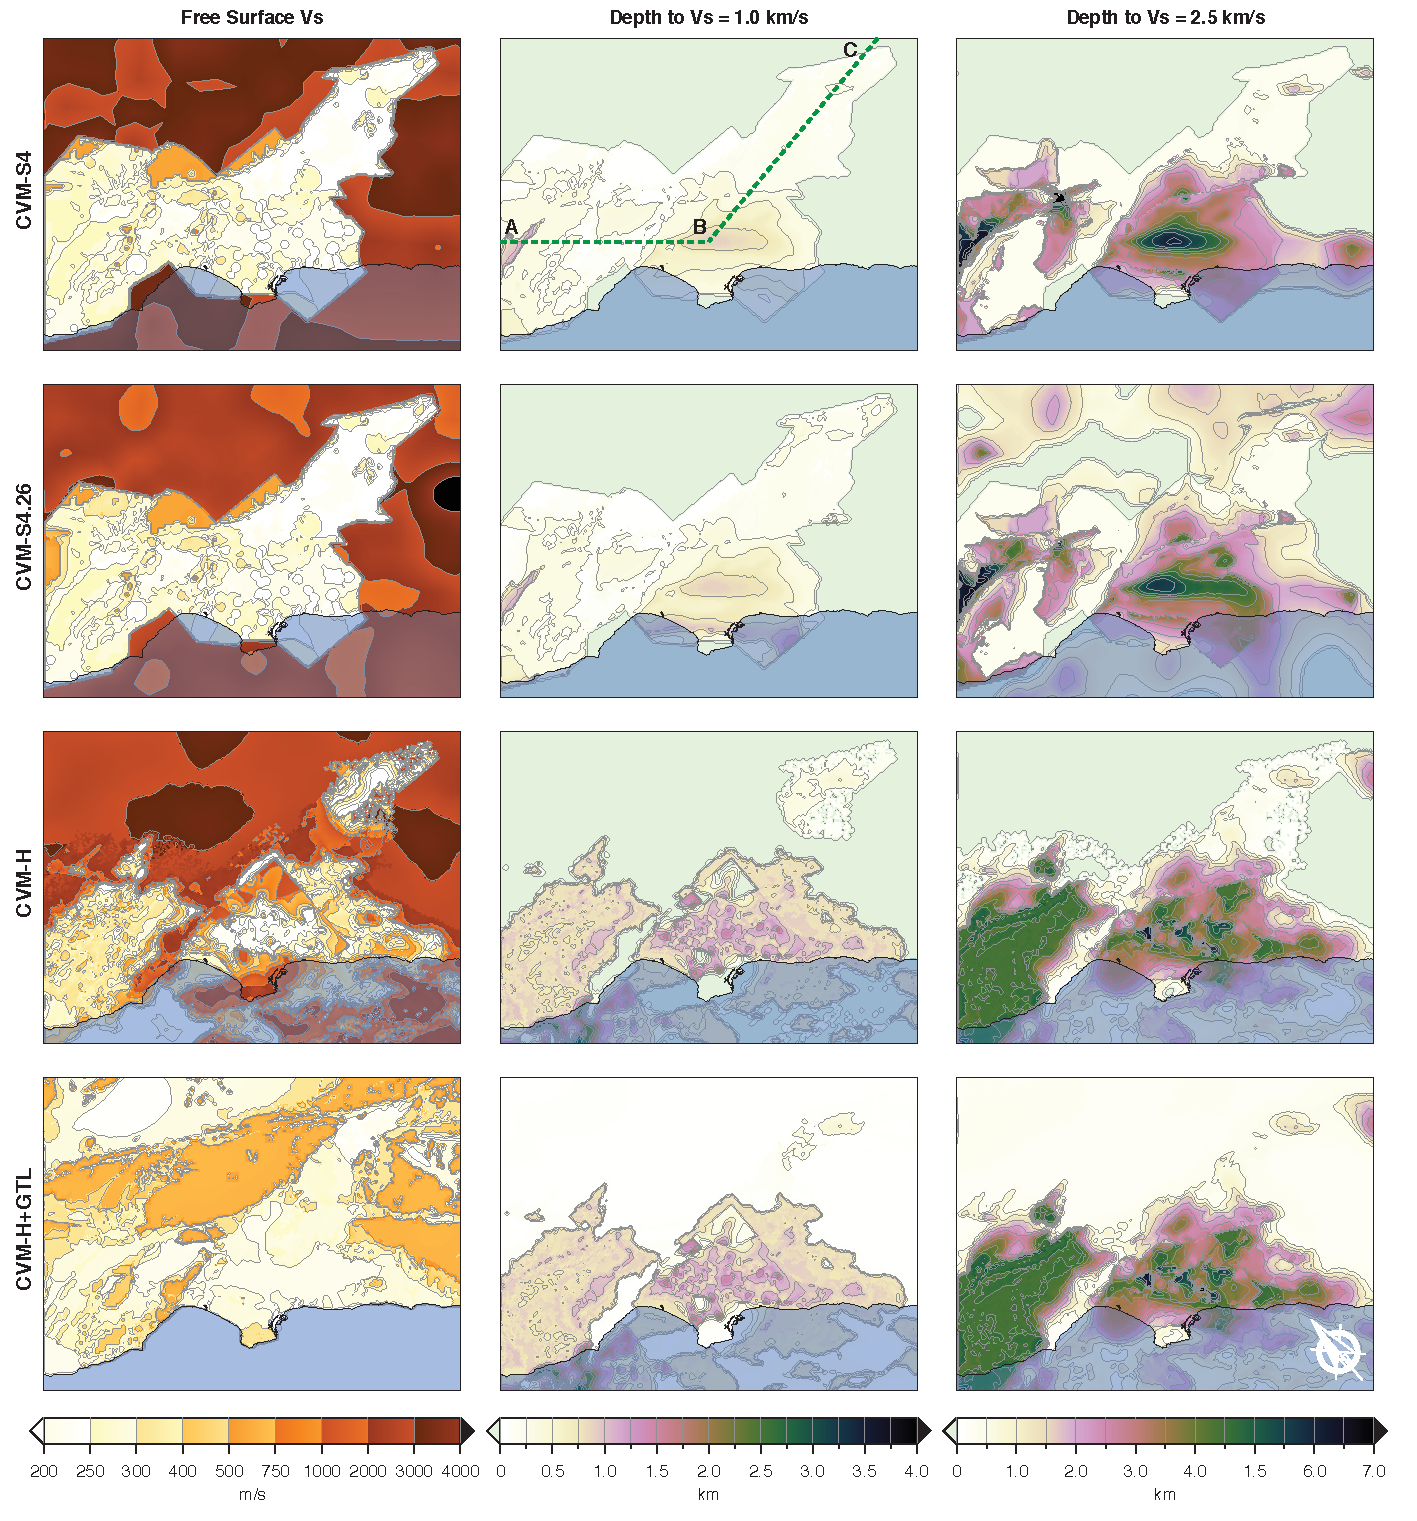
\includegraphics
        [width=\textwidth]
        {figures/pdf/figure-02}
    \caption{Comparison between the southern California community velocity models considered. Left: free-surface shear wave velocity, \vs{}. Center: depth to the isosurface at which \vseq{1000}. Right: depth to the isosurface at which \vseq{2500}. }
    \label{fig:hslices}
\end{figure*}
